\section*{\hypertarget{gameplay}{Reglas}}
"Si quieres calma, mejor toma el siguiente tren".\\
\indent -- Lightning

\begin{center} 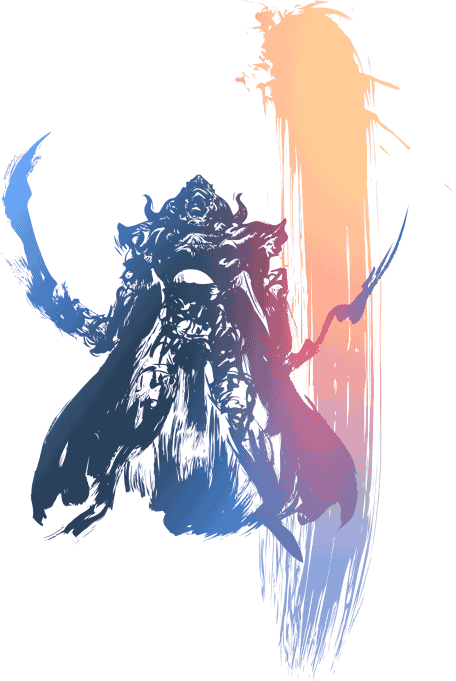
\includegraphics[width=\columnwidth]{./art/images/ff12.png} \end{center}

\addcontentsline{toc}{section}{Reglas}

\subsubsection*{Introducción}
Final Fantasy es una serie de videojuegos que han dado forma al género desde su primer lanzamiento en 1987. Aunque cada título de Final Fantasy cuenta con su historia, entorno y personajes únicos, se perciben como parte de la misma serie. Esto no solo se debe a los muchos elementos recurrentes que tienen en común, sino también porque las historias se centran en un grupo de héroes que afrontan un gran conflicto. \mbox{\textbf{Omega Fantasy}} es un sistema de juego de rol de mesa que te ayuda a ti y a tus amigos a crear y jugar en una aventura de Final Fantasy propia.

\vfill

\subsubsection*{Primeros pasos}
Para jugar a Omega Fantasy solo necesitas dados, papel, bolígrafos, este libro y al menos un amigo más, pero se recomienda un grupo de 4 a 6. Elijan a una persona para convertirse en \mbox{\textbf{Director del Juego}}, que crea el mundo de fantasía y narra la aventura. Cada uno es un \textbf{Jugador}, que toma el papel de uno de los protagonistas. No necesitas ningún conocimiento previo de Final Fantasy ni experiencia jugando rol. Todo lo necesario se explica aquí.

\pagebreak

\subsubsection*{Jugadores}
Los jugadores crean e interpretan \textbf{personajes} que son los protagonistas de la historia. Toman el papel de sus personajes y juegan el juego desde su perspectiva. Estos aventureros viajan juntos como \textbf{grupo}, exploran el mundo, interactúan con las personas y luchan contra los enemigos. Normalmente, el grupo se enfrenta a un \textbf{conflicto central} creado por el Director del Juego, que será el objetivo general de su aventura. Este libro incluye varias reglas y opciones que ayudan a crear y desarrollar a los personajes.

\subsubsection*{Director del Juego}
El Director del Juego (abreviado \textbf{DJ}) crea el mundo en el que tiene lugar la aventura utilizando el contenido y las directrices de este libro. Durante el juego, describe el entorno al grupo y cómo reacciona a sus acciones. El DJ asume el papel de todos los personajes no jugadores para narrar las conversaciones y combates. Las reglas de este libro ayudan al DJ a determinar el resultado de algunas acciones, aunque a menudo debe decidir por sí mismo.

\subsubsection*{Dados}
Las tiradas de dados se utilizan en diversas situaciones para ayudar a decidir el resultado de ciertas acciones. Sin embargo, dependiendo del contexto, la naturaleza exacta de dicha tirada puede diferir. Los únicos dados utilizados en este juego son los estándares de seis caras y a menudo usamos \textbf{d} para referirnos a dicho dado. Además, usamos por ejemplo "4d" para describir una tirada de 4 dados, donde el resultado es la suma de todos los dados tirados.

\vspace{1cm}

\example{Roleo}
{
\begin{description}[leftmargin=*]
 \item[Hironobu (Director del Juego):] Llegan a las Llanuras del Trueno, que es un vasto páramo cubierto por niebla gruesa y nubes oscuras. Los lugareños irguieron torres que actúan como pararrayos, pero observan que los rayos a menudo caen sobre campo abierto.
 \item[Yoshinori (jugando como Wakka):] Nos dirigimos hacia el norte, ni muy cerca ni muy lejos de las torres, ¿sí?
 \item[Nobuo (jugando como Rikku):] ¡Quiero ir a casa! ¡Odio los rayos! ¡Odio los truenos!
 \item[Tetsuya (jugando como Auron):] Esta tormenta no para. Mejor cruzar rápidamente.
 \item[Hironobu (Director del Juego):] También pueden ver un pequeño edificio cerca. Parece ser una posada.
 \item[Nobuo (jugando como Rikku):] ¡Vayamos allí! ¡Por favor! ¡Soy demasiado joven para morir!
 \item[Tetsuya (jugando como Auron):] Bien, descansemos. Ella es peor que la tormenta.
\end{description}
}

\pagebreak
